% !TEX TS-program = pdflatexmk
\documentclass[12pt]{article}

% Layout.
\usepackage[top=.75in, bottom=0.75in, left=.75in, right=.75in, headheight=1in, headsep=6pt]{geometry}

% Fonts.
\usepackage{mathptmx}
\usepackage[scaled=0.86]{helvet}
\renewcommand{\emph}[1]{\textsf{\textbf{#1}}}

% Misc packages.
\usepackage{amsmath,amssymb,latexsym}
\usepackage{graphicx,tikz}
\usepackage{array}
\usepackage{xcolor}
\usepackage{multicol}
\usepackage{tabularx,colortbl}
\usepackage{enumitem}
%to make tikz pics work
\usepackage{tikz,pgfplots}
\usetikzlibrary{arrows}
\newcommand{\midarrow}{\tikz \draw[-triangle 90] (0,0) -- +(.1,0);}

\usepackage[colorlinks=true]{hyperref}

% Paragraph spacing
\parindent 0pt
\parskip 6pt plus 1pt
\def\tableindent{\hskip 0.5 in}
\def\ts{\hskip 1.5 em}

\usepackage{fancyhdr}
\pagestyle{fancy} 
\lhead{\large\sf\textbf{MATH 663 }}
\rhead{\large\sf\textbf{Fall 2023}}
\chead{\large\sf\textbf{HW 8 }}

\newcommand{\localhead}[1]{\par\smallskip\textbf{#1}\nobreak\\}%
\def\heading#1{\localhead{\large\emph{#1}}}
\def\subheading#1{\localhead{\emph{#1}}}

%% Special Math Symbol shortcuts
\newcommand{\bbN}{\mathbb{N}}
\newcommand{\rad}{\text{rad}}
\newcommand{\diam}{\text{diam}}

%\newenvironment{clist}%
%{\bgroup\parskip 0pt\begin{list}{$\bullet$}{\partopsep 4pt\topsep 0pt\itemsep -2pt}}%
%{\end{list}\egroup}%

\usetikzlibrary{calc,arrows.meta}
%\pgfplotsset{my style/.append style={axis x line=middle, axis y line=
%middle, xlabel={$x$}, ylabel={$y$}, axis equal }}


\begin{document}
\begin{enumerate}
	\item Give an example to show that if $G$ is allowed to have multiple edges, then $\chi'(G)$ may exceed $\Delta(G) +1.$
	\item Without using Proposition 5.3.1, show that $\chi'(G) =k$ for every $k$-regular bipartite graph $G.$
	\item Give an explicit edge-coloring to prove that the $n$-dimensional cube, $Q^n$, is Class 1.
	\item Prove that if $G$ is a regular graph with a cut vertex, then $\chi'(G) > \Delta(G).$
	\item The \emph{cartesian product} of two graph $G$ and $H$, denoted $G \: \square \: H,$
	is the graph with vertex set $V(G \: \square \: H)=V(G) \times V(H).$ A pair of vertices $(x_1,y_1), (x_2,y_2)$ are adjacent in  $G \: \square \: H$ if and only if $x_1=x_2$ and $y_1y_2 \in E(H)$ or $x_1x_2 \in E(G)$ and $y_1=y_2.$
	\begin{enumerate}
	\item Draw $P_2 \: \square \: C^3.$
	\item Prove that $\Delta(G \: \square \: H)= \Delta(G) + \Delta(H)$
	\item Prove that if $\chi'(H)=\Delta(H)$, then $\chi'(G \: \square \: H)=\Delta(G \: \square \: H).$
	\end{enumerate}
	\item
	\begin{enumerate}
	\item Let $G_1$ be a 5-cycle with one chord. Show that there exists a graph $H$ such that $L(H)=G_1.$
	\item Prove that for the graph $G_2$ (drawn below) that there does not exist any graph $H$ such that $L(H)=G_2.$\\
	
	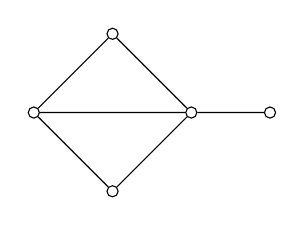
\begin{tikzpicture}[scale=1,every node/.style={draw,circle, inner sep=.05 cm}]
\foreach \i in {0,1,2,3}{
	\node (\i) at (\i*90:1){};
	}
\node (5) at (0:2){};
\draw (5)--(0)--(1)--(2)--(3)--(0)--(2);
\end{tikzpicture}	
	\end{enumerate}
\end{enumerate}
\end{document}